\begin{figure}[H]
  \centering
  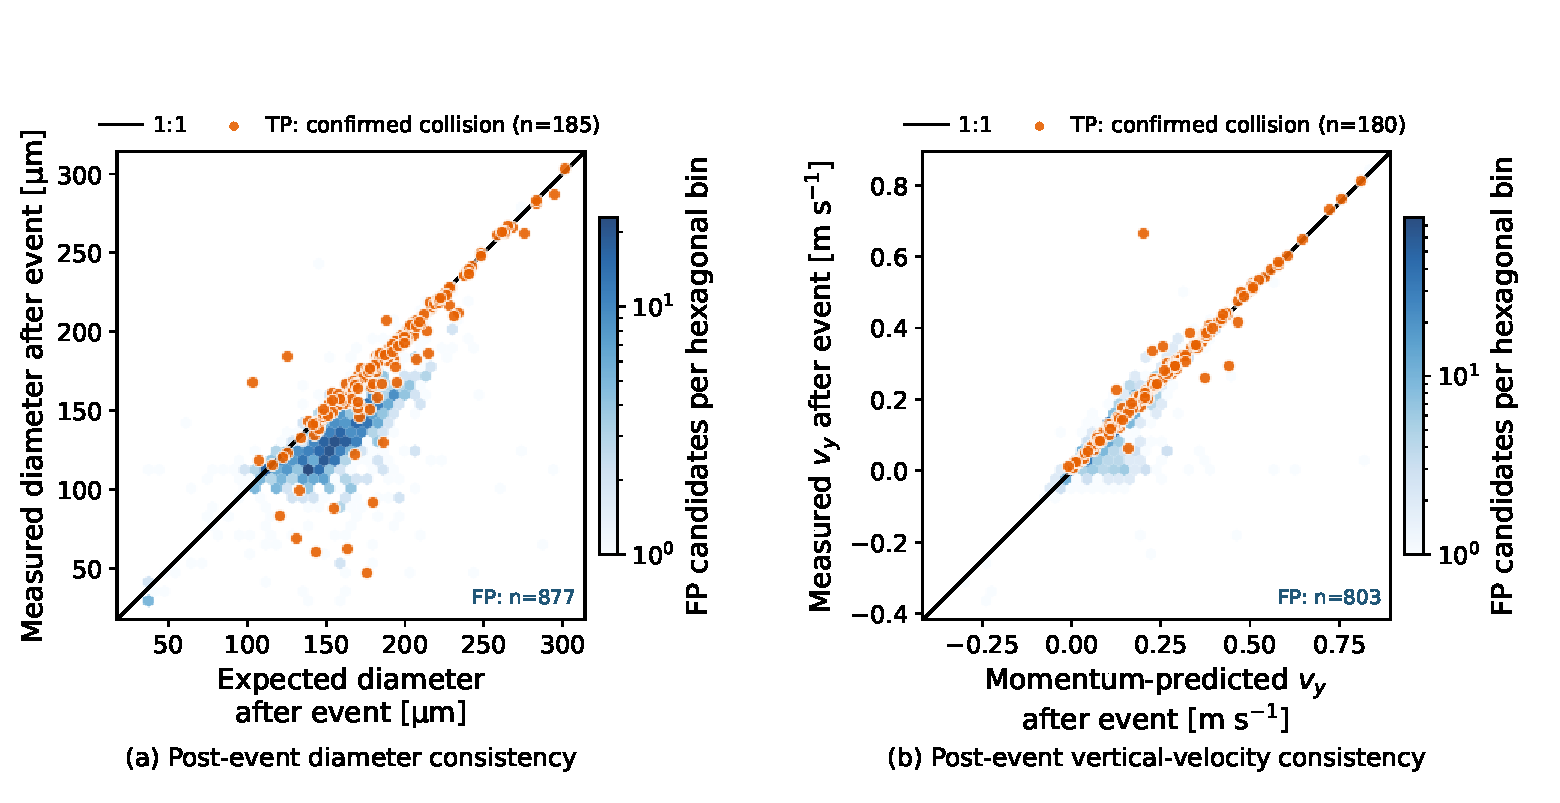
\includegraphics[width=\linewidth]{figures/expresult/physical_consistency_combined_260715.pdf}
  \caption{Physical-consistency diagnostics for visually reviewed experimental candidates. (a) Measured post-event diameter versus the volume-conservation prediction, \(D_{\mathrm{exp}}=(D_1^3+D_2^3)^{1/3}\). (b) Measured post-event vertical velocity versus the momentum-conservation prediction, \(v_{y,\mathrm{exp}}=(D_1^3v_{y,1}+D_2^3v_{y,2})/(D_1^3+D_2^3)\), with downward velocity positive. Orange markers show confirmed events: 185 in (a) and 180 with valid velocity estimates in (b). Blue hexagonal bins show the numbers of rejected candidates on logarithmic color scales. Black lines indicate one-to-one agreement.}
  \label{fig:experimental_physical_consistency}
\end{figure}
